\section{EKG-Schaltung mit AD627}
\subsection{Aufgabenstellung}
Die Schaltung soll für eine untere Grenzfrequenz von ca. 0,1Hz und einer oberen Grenzfrequenz von ca. 30Hz dimensioniert werden. Die Gesamtverstärkung soll ca. 200 betragen. Die erste Stufe soll ein Gain von kleiner 100 haben. Die Versorgungsspannung soll $\pm5\V$ betragen und der Eingangsfilter soll laut Datenblatt des AD627 dimensioniert werden. Die nachfolgende Sallen-Key Stufen soll dann auf 30Hz ausgelegt werden. hier kann die im vorherigen Kapitel dimensionierte Schaltung verwendet werden.

\begin{figure}[H]
    \centering
    \scalebox{0.75}{
    \begin{circuitikz}[]
        \draw (-8.5,0.5) node[inst amp ra](instamp){AD627};
        \draw (instamp.ra+) to[R=$R_4$] (instamp.ra-);
        \draw (instamp.-) to[R=$R_3$] ++(0,2) node[ground, yscale=-1]{};
        \draw (instamp.-) to[short,*-] ++(-2,0) to[C=$C_3$] ++(0,2) node[ground, yscale=-1]{};
        \draw (instamp.-) to[short,*-] ++(-2,0) to[C=$C_1$] ++(-2,0) to[R=$R_1$,-o] ++(-2,0) node[left]{Grün};

        \draw (instamp.+) to[R=$R_5$] ++(0,-2) node[ground]{};
        \draw (instamp.+) to[short,*-] ++(-2,0) to[C=$C_5$] ++(0,-2) node[ground]{};
        \draw (instamp.+) to[short,*-] ++(-2,0) to[C=$C_2$] ++(-2,0) to[R=$R_2$,-o] ++(-2,0) node[left]{Rot};

        \draw (instamp.-) to[short,*-] ++(-2,0) to[C=$C_4$,*-*] ++(0,-2.85);
        
        \draw (-16,-3) node[left] {Gelb} to[short,o-]++(1,0) to[short]++(0,-1) node[ground]{};
        
        \draw (instamp.refv down) to[short] ++(0,-1) node[ground]{};
        
        \draw (0,0) node[op amp,yscale=-1] (opamp) {\scalebox{1}[-1]{$AD823$}};
        \draw (opamp.down) --++(0,0.5) node[vcc]{$V_{CC}$};
        \draw (opamp.up) --++(0,-0.5) node[vee]{$V_{EE}$};
        
        \draw (opamp.+) to[short, -*] ++(-2,0)
            to[C=$C_7$] ++(0,-2) node[ground]{};
        \draw (opamp.+) to[short, -*] ++(-2,0)
            to[R=$R_7$] ++(-2,0)
            to[R=$R_6$] ++(-2,0);
        \draw (-5.25,0.5) to[short,*-] ++(0,2)
            to[C=$C_6$] ++(7.445,0)
            to[short] ++(0,-2.5)
            to[short] (opamp.out);
        \draw (opamp.out) to[short,-*] ++(1,0)
            to[R=$R_9$,-*] ++(0,-3)
            to[R=$R_8$] ++(0,-2) node[ground]{};
        \draw (2.2,-3) to[short] ++(-4,0)
            to[short] ++(0,2.5)
            to[short] (opamp.-);
        \draw (opamp.out) to[short,-o] ++(2,0) node[right] {$U_{out}$};
        \end{circuitikz}
        }
    \caption{EKG-Verstärker}
    \label{fig:Schalt_EKG_Verst}
 \end{figure}

\subsection{Auslegung der Schaltung}
Hier wurde aus Gründen der Übersichtlichkeit auf eine Darstellung verzichtet, außerdem können die Bauteilwerte für die Sallenkey Filterstufe aus dem vorherigen Kapitel entnommen werden.
\begin{table}[H]
\centering
\caption{Bauteilwerte EKG-Verstärker}
\label{tab:Vals_EKG_Verst}
\begin{tabular}{|l|l|l|}
\hline
\rowcolor[HTML]{C0C0C0} 
Bauteil & berechnet      & gewählt     \\ \hline
$R_1$   & $120,57\KOhms$ & $120\KOhms$ \\ \hline
$R_2$   & $120,57\KOhms$ & $120\KOhms$ \\ \hline
$R_3$   &                & $8,2\MOhms$ \\ \hline
$R_4$   & $40\KOhms$     & $39\KOhms$  \\ \hline
$R_5$   &                & $8,2\MOhms$ \\ \hline
$C_1$   & $194,09\nF$    & $220\nF$    \\ \hline
$C_2$   & $194,09\nF$    & $220\nF$    \\ \hline
$C_3$   & $4,4\nF$       & $4,7\nF$    \\ \hline
$C_4$   &                & $22\nF$     \\ \hline
$C_5$   & $4,4\nF$       & $4,7\nF$    \\ \hline
\end{tabular}
\end{table}

\subsection{Messergebnisse}
\begin{figure}[h]
    \centering
    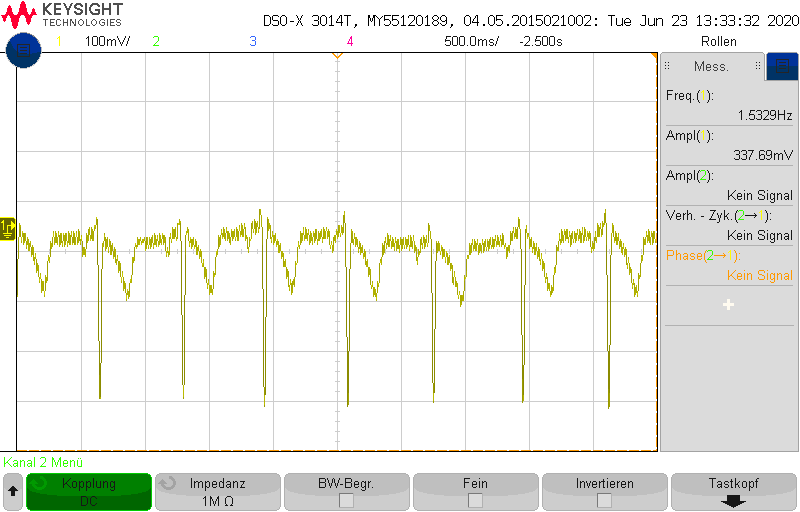
\includegraphics[width = \costumPicWidth]{Lab_4/Messungen/ekg.png}
    \caption{Ableitung des EKG am Autor}
    \label{fig:my_label}
\end{figure}
\begin{figure}[h]
    \centering
    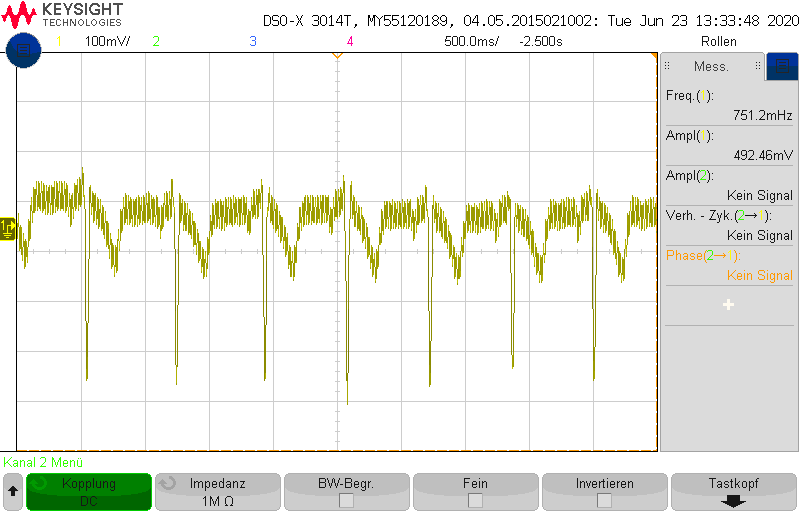
\includegraphics[width = \costumPicWidth]{Lab_4/Messungen/ekg3.png}
    \caption{Ableitung des EKG am Autor, mit Netzkabel}
    \label{fig:EKG_Kabel}
\end{figure}
Während der Messung welche in \autoref{fig:EKG_Kabel} zu sehen ist, umfasst der Proband mit einer Hand ein Netzkabel welches an der Steckdose angeschlossen war. Das Kabel war jedoch an keinem Gerät angeschlossen, dass heißt dass keine signifikanten Ströme flossen. Trotzdem ist zu sehen, dass hier eine nicht zufriedenstellende Unterdrückung des 50Hz Netzsinus stattfindet und hier die entweder die Grenzfrequenz herabgesetzt werden muss, oder mit einem digitalen Filter nachbearbeitet werden sollte.
\begin{figure}[h]
    \centering
    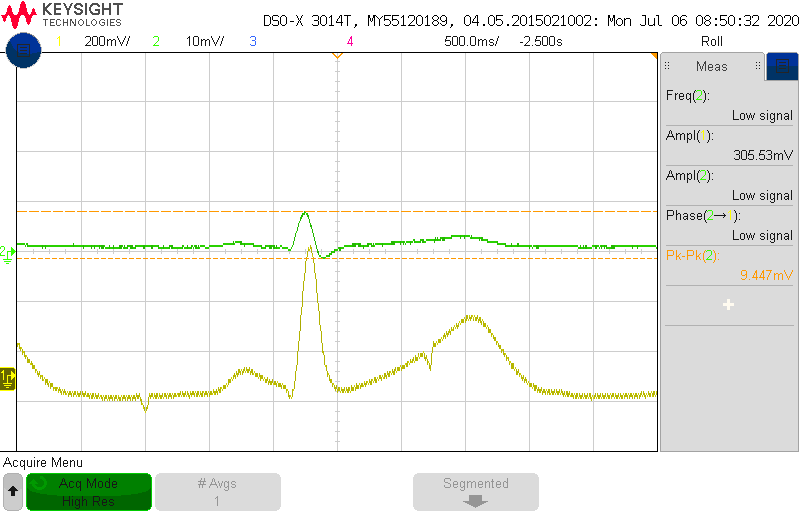
\includegraphics[width = \costumPicWidth]{Lab_4/Messungen/ekg.waveform.png}
    \caption{EKG Verstärker mit Cardiac Funktion des Signalgenerators}
    \label{fig:my_label}
\end{figure}
\begin{figure}[h]
    \centering
    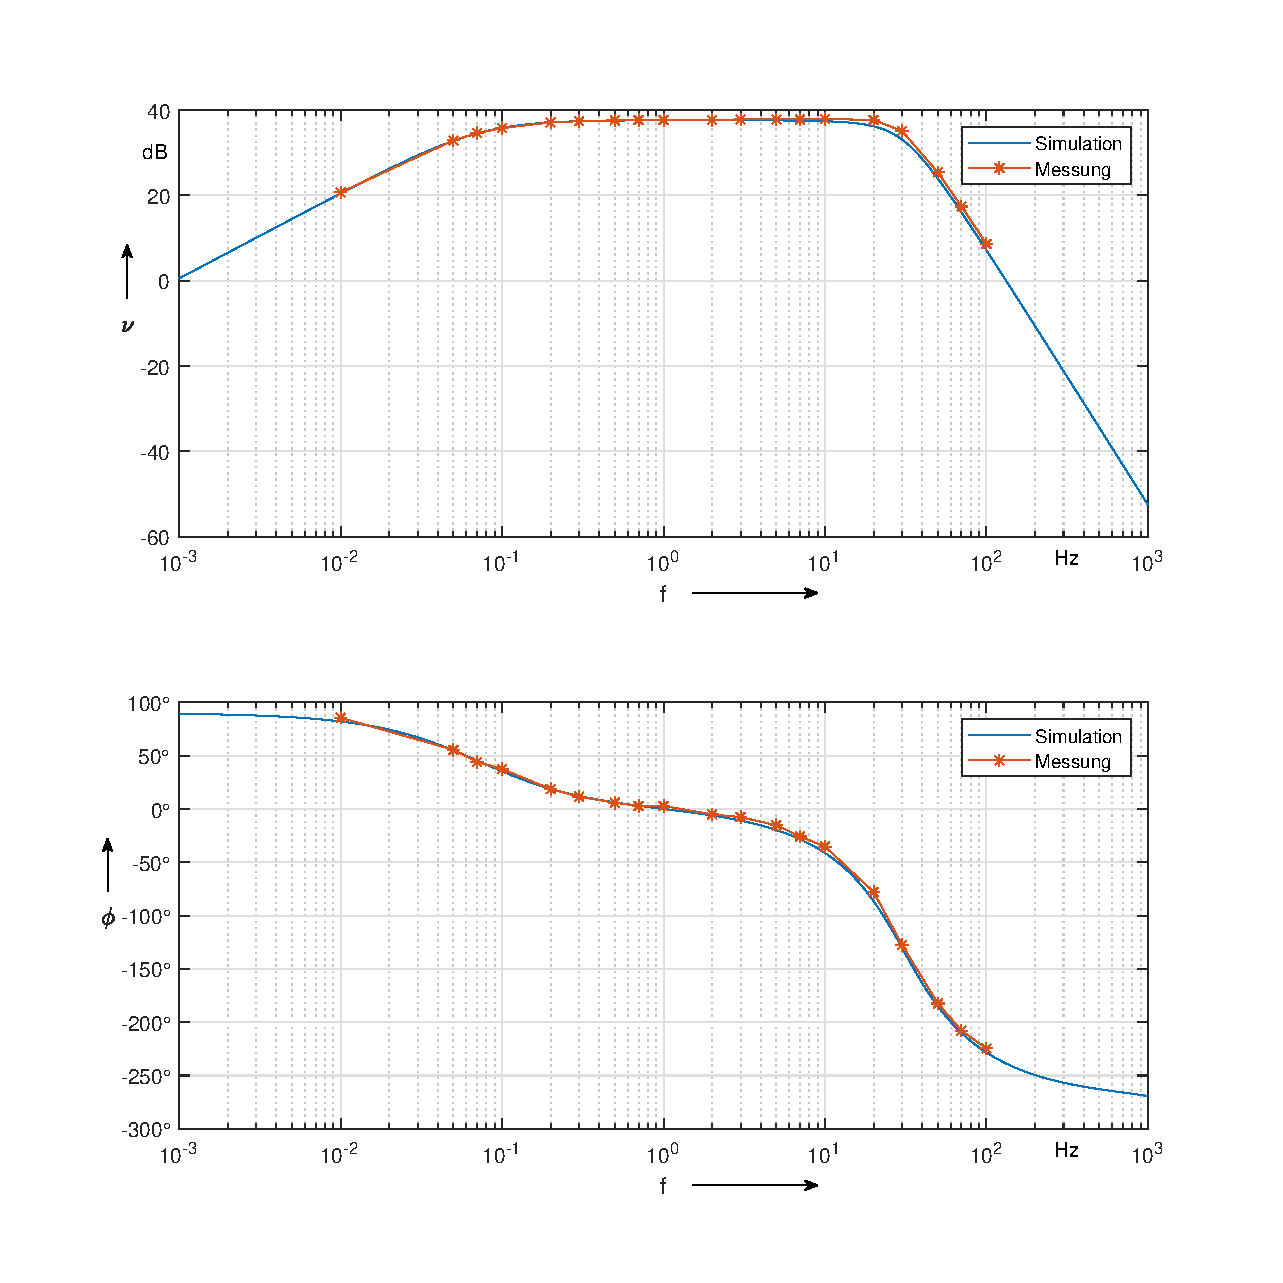
\includegraphics[width = \costumPicWidth]{Lab_4/Plots/EKG.eps}
    \caption{Bodediagramm des EKG-Verstärkers}
    \label{fig:bode_ekg}
\end{figure}
\